% ======================================================================
% Q-DARE -- consolidated revised draft for IEEE ISCAS 2027
%
% This version follows the latest discussion:
%   1) ViDA is reimplemented and evaluated in the SAME cycle-level simulator.
%   2) A100 comparison follows EXION-style compute-matched scaling.
%   3) Naive Cache+Quant is added as the direct QAC ablation.
%   4) QAC description is made more reproducible without expanding the paper much.
%   5) Q-DARE now uses the complete TSMC 7-nm synthesis result,
%      including logic and SRAM macros: 1.051 mm^2 and 614.4 mW.
%      The resulting ViDA-normalized area efficiency is 2.81x.
%
% REQUIRED BEFORE SUBMISSION:
%   - Fill \NaiveCQVBench.
%   - Fill the four compact QAC implementation macros below.
%   - Update fig/gen_img.pdf to add the Naive Cache+Quant row.
%   - In Fig. 2, optionally add "QAC Cache/Reuse Ctrl." inside Global Controller.
%   - Check Fig. 3 cycle labels: 0--3, 4--7, 8--11, 11--14
%     (if contiguous chunks are intended, the last should be 12--15).
% ======================================================================

\documentclass[conference]{IEEEtran}

\usepackage{cite}
\usepackage{amsmath,amssymb}
\usepackage{graphicx}
\graphicspath{{../}}
\usepackage{booktabs}
\usepackage{xcolor}
\usepackage{array}
\usepackage{multirow}
\usepackage{url}

% ----------------------------------------------------------------------
% Fill these after the final QAC characterization.
% They are intentionally centralized so no result is silently invented.
% ----------------------------------------------------------------------
\newcommand{\NaiveCQVBench}{\textcolor{red}{XX.XX}}
\newcommand{\QACFeatureDesc}{\textcolor{red}{[exact feature tensor/location]}}
\newcommand{\QACQuantDesc}{\textcolor{red}{[quantizer granularity/scale]}}
\newcommand{\QACMapDesc}{\textcolor{red}{[form of $g_q$: LUT/polynomial/etc.]}}
\newcommand{\QACCalibDesc}{\textcolor{red}{[calibration set and target]}}

% Final reported values used in the current manuscript.
\newcommand{\QDAREStepGeoA}{10.96}
\newcommand{\QDAREEnergyGeoA}{26.59}
\newcommand{\QDAREViDAThroughputGeo}{1.06}
\newcommand{\QDAREViDAAreaGeo}{2.04}

\title{Q-DARE: Quantization-Aligned Caching with a\\
Dimension-Adaptive Reconfigurable Engine for\\
Video Diffusion Transformers}

\author{
\IEEEauthorblockN{
Enhao Tang, Wei Li, Faxun Jin, and Jun Lin$^{*}$
}
\IEEEauthorblockA{
\textit{School of Electronic Science and Technology, Nanjing University, Nanjing, China}\\
$^{*}$Corresponding author: Jun Lin (jlin@nju.edu.cn)
}
}

\begin{document}
\maketitle

\begin{abstract}
Video Diffusion Transformers (VDiTs) repeatedly execute expensive spatial--temporal transformer blocks during denoising. Caching and quantization reduce the number and cost of recomputed steps, but their naive composition creates two mismatches: full-precision cache indicators need not reflect quantized execution, and asymmetric spatial/temporal attention shapes underutilize fixed-width arrays. We present \textbf{Q-DARE}, an algorithm--hardware co-design combining \emph{quantization-aligned caching} (QAC) with a \emph{dimension-adaptive reconfigurable engine} (DARE). QAC evaluates cache relevance in the quantized domain, while DARE adapts the output axis of $QK^{\mathsf T}$ and the reduction axis of $PV$ on one shared datapath. Experimental results on Open-Sora v1.2 show that Q-DARE achieves
a VBench score of 76.61 versus 76.77 for FP16. Across 64--512-frame workloads, Q-DARE achieves \QDAREStepGeoA$\times$ geomean STDiT step-throughput and \QDAREEnergyGeoA$\times$ energy-efficiency improvement over A100, while reaching \QDAREViDAThroughputGeo$\times$ geomean video throughput and \QDAREViDAAreaGeo$\times$ geomean area efficiency over ViDA,
a state-of-the-art VDiT accelerator.
\end{abstract}

\begin{figure*}[t]
  \centering
  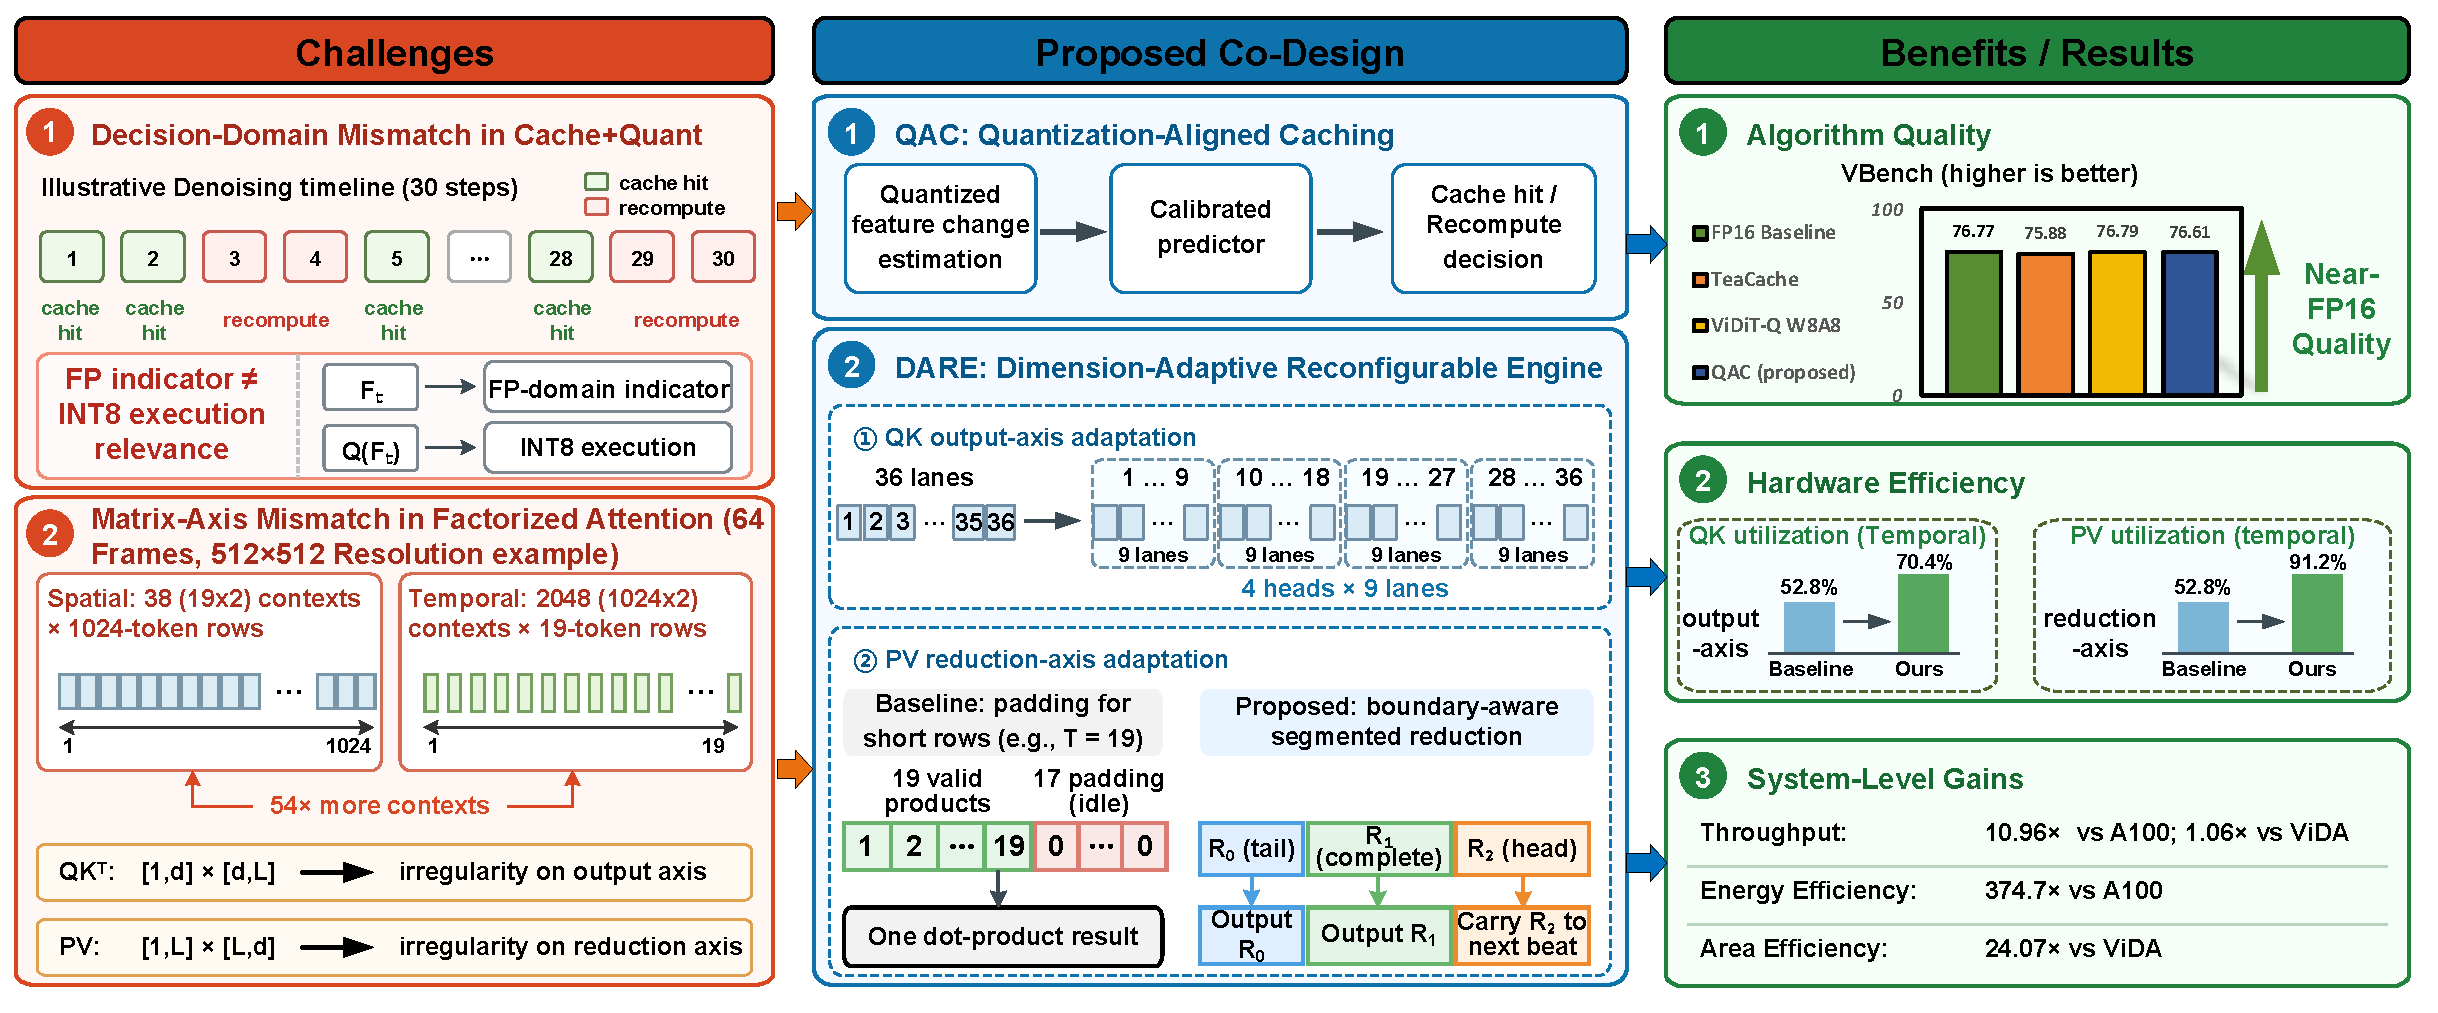
\includegraphics[width=\textwidth]{fig/overview.pdf}
  \caption{Q-DARE co-design overview using a 64-frame, $512\times512$ resolution example ($T=19$, $S=1024$ after VAE tokenization, with an effective batch size of 2 for classifier-free guidance): QAC aligns cache decisions with quantized execution, while DARE adapts the shared attention datapath to spatial/temporal shape asymmetry.}
  \label{fig:overview}
  \vspace{-4mm}
\end{figure*}

% ======================================================================
\section{Introduction}
\label{sec:intro}

\IEEEPARstart{D}{iffusion} Transformers (DiTs) have emerged as scalable
backbones for generative modeling~\cite{peebles2023dit}.
Recent Video Diffusion Transformers (VDiTs) extend this design to
spatio-temporal token processing~\cite{ma2025latte,zheng2024opensora}.
Their iterative denoising repeatedly evaluates expensive
Spatial-Temporal Diffusion Transformer (STDiT) blocks; Open-Sora v1.2,
for example, executes 28 spatial--temporal block pairs over 30 sampling
steps~\cite{zheng2024opensora}. Timestep caching skips redundant STDiT evaluations~\cite{liu2025teacache}, whereas post-training quantization reduces the cost of each recomputed step~\cite{zhao2025viditq}. Recent joint methods further optimize cache schedules, correction, or precision selection~\cite{liu2025cachequant,wu2025quantcache}, while hardware accelerators exploit adaptive dataflow or inter-iteration redundancy~\cite{ding2025vida, kim2025ditto, heo2025exion}. However, combining caching with quantized execution still exposes two cross-layer mismatches.

% These optimizations attack different dimensions of cost, but their direct composition leaves two cross-layer mismatches.

First, a \textbf{decision-domain mismatch} arises when a full-precision (FP) cache indicator ranks timestep changes that are later altered by quantization. Quantization is nonlinear and piecewise constant: an FP difference may disappear inside one quantization bin, while a smaller change may cross a bin boundary. Thus an FP-domain indicator can mis-rank the value of recomputation once the actual execution path is quantized.

Second, a \textbf{matrix-axis mismatch} arises because Open-Sora's factorized spatial/temporal attention~\cite{zheng2024opensora} places the varying sequence dimension on different GEMM axes. In $QK^{\mathsf T}$ it determines the output width, whereas in $PV$, with $P$ denoting the post-softmax attention matrix, it becomes the reduction length. Our 64-, 256-, and 512-frame workloads have temporal lengths $T=19$, 76, and 151, respectively. For the representative $T=19$ case, mapping one head to all 36 lanes fragments the $QK^{\mathsf T}$ output, while row-wise padding wastes the same array in $PV$.

Fig.~\ref{fig:overview} summarizes \textbf{Q-DARE}. \textbf{Quantization-aligned caching (QAC)} evaluates cache relevance in the same numerical domain as recomputation and calibrates the indicator against the quantized trajectory, aligning \emph{which} steps are recomputed. The \textbf{dimension-adaptive reconfigurable engine (DARE)} improves \emph{how} those steps execute by reusing one processing-element array (PEA): temporal $QK^{\mathsf T}$ changes output-lane ownership, whereas temporal $PV$ packs boundary-tagged reductions and replays $V$ without an explicit transpose. QAC and DARE are therefore complementary: the former removes unnecessary STDiT executions, while the latter improves utilization of the remaining ones.

Experimental results on Open-Sora v1.2 show that Q-DARE achieves
a VBench score of 76.61 versus 76.77 for FP16. For $T=19$, DARE raises temporal $QK^{\mathsf T}$ lane utilization from 52.8\% to 70.4\% and temporal $PV$ product utilization from 52.8\% to 91.2\%. Across 64--512-frame workloads, Q-DARE achieves \QDAREStepGeoA$\times$ geomean STDiT step throughput and \QDAREEnergyGeoA$\times$ energy efficiency over A100, and \QDAREViDAThroughputGeo$\times$ geomean video throughput with \QDAREViDAAreaGeo$\times$ area efficiency over ViDA.

Our contributions are summarized as follows:
\begin{itemize}
  % \item We identify a decision-domain mismatch in Cache+Quant and introduce QAC, a lightweight mechanism that aligns cache decisions with quantized execution while preserving the baseline cache policy.
  \item We identify an indicator--execution domain mismatch in Cache+Quant and propose QAC, which aligns cache decisions with quantized execution without changing the baseline cache policy.
  \item We design DARE, a shared datapath that adapts the output and reduction axes of factorized attention without duplicating the PEA.
  \item Extensive evaluations demonstrate that Q-DARE achieves near-FP16 quality with substantial throughput and efficiency gains.
\end{itemize}

% ======================================================================
\section{Quantization-Aligned Caching}
\label{sec:qac}

\subsection{Decision-Domain Mismatch}

Let $F_t$ denote the AdaLN-modulated input to the first spatial
Transformer block at denoising step $t$.
Conventional timestep caching, such as TeaCache~\cite{liu2025teacache},
measures its normalized full-precision (FP) variation,
\begin{equation}
d_t^{\mathrm{FP}}=
\frac{\lVert F_t-F_{t-1}\rVert_1}
     {\lVert F_{t-1}\rVert_1+\epsilon}.
\label{eq:fp_indicator}
\end{equation}
The predictor is therefore calibrated on an FP trajectory, whereas
recomputed steps follow quantized execution.
Since quantization can collapse nearby FP values into the same integer
code or move a smaller change across a quantization boundary,
$d_t^{\mathrm{FP}}$ need not preserve the relative importance of
recomputation.
Because the cache rule accumulates predicted variation until a threshold
crossing, such reordering can alter both cache hits and refresh points.

\subsection{Quantization-Aligned Indicator}

QAC evaluates the same feature in the quantized execution domain.
The recomputation path uses symmetric INT8 quantization with offline
per-channel weight scales and online per-token activation scales.
For $F_t$, the dynamic activation scale is
\begin{equation}
s_{b,n}=\frac{\max_c |F_{t,b,n,c}|}{127},
\end{equation}
and QAC forms
\begin{equation}
\widetilde F_t=D(Q_s(F_t)),\qquad
d_t^{\mathrm Q}=
\frac{\lVert\widetilde F_t-\widetilde F_{t-1}\rVert_1}
     {\lVert\widetilde F_{t-1}\rVert_1+\epsilon},
\label{eq:q_indicator}
\end{equation}
where $Q_s(\cdot)$ and $D(\cdot)$ denote symmetric INT8 quantization
and dequantization.
Thus the cache indicator experiences the same rounding and clipping
effects as the activation execution path without requiring an FP
recomputation path.

\subsection{Calibration and Runtime Policy}

QAC maps the inexpensive feature variation to the change of the full
STDiT residual using a fourth-order polynomial,
\begin{equation}
\widehat r_t^{\mathrm Q}=g_q(d_t^{\mathrm Q}).
\label{eq:qac_mapping}
\end{equation}
% The polynomial is fitted offline using 100 randomly sampled VBench
% prompts \cite{huang2024vbench}.
The polynomial is fitted offline using 100 disjoint VBench calibration prompts \cite{huang2024vbench}.
For each adjacent timestep pair, the calibration target is the
normalized change of the residual across all 28 Transformer blocks,
\begin{equation}
R_t=x_t^{\mathrm{after}}-x_t^{\mathrm{before}},\qquad
r_t=
\frac{\lVert R_t-R_{t-1}\rVert_1}
     {\lVert R_{t-1}\rVert_1+\epsilon}.
\end{equation}
The resulting $g_q$ therefore predicts the expensive full-block
variation from the low-cost quantized feature change.

At runtime, $\widehat r_t^{\mathrm Q}$ is accumulated by the baseline
thresholded cache rule.
Cached states are reused while the accumulated variation remains within
the reuse budget; once the budget is exceeded, STDiT is recomputed and
the cached state is refreshed. QAC only determines cache/recompute decisions; recomputed steps follow the same quantized execution path accelerated by DARE.

% The Instruction / Global Controller only issues a cache/recompute
% decision, while recomputed steps enter the same quantized datapath
% accelerated by DARE.

\begin{figure*}[!t]
  \centering
  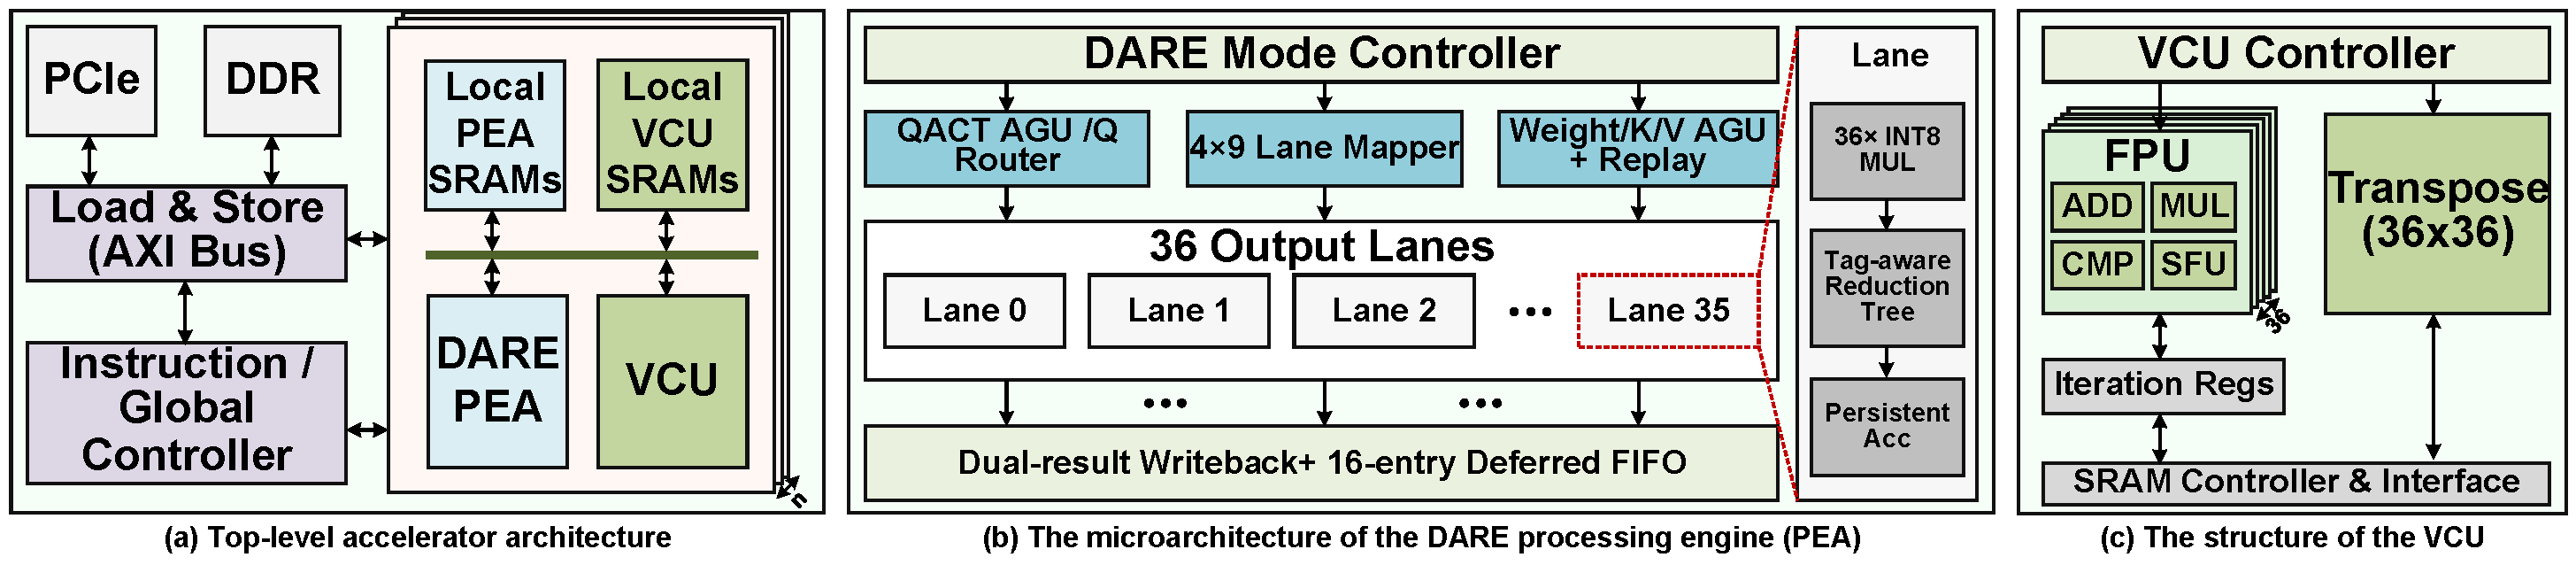
\includegraphics[width=\textwidth]{fig/hardware-overview.pdf}
  \caption{DARE hardware organization: (a) top-level architecture;
  (b) the adaptive PEA; and (c) the FP16 VCU.}
  \label{fig:dare_arch}
  \vspace{-4mm}
\end{figure*}
% ======================================================================
% !TEX root = ../main.tex

\section{DARE: Dimension-Adaptive Reconfigurable Engine}
\label{sec:hardware}

\subsection{Architecture and Core Organization}

Fig.~\ref{fig:dare_arch}(a) shows the accelerator organization.
Each core consists of a DARE processing-element array (PEA), a vector
compute unit (VCU), and their local SRAMs.
The $36\times36$ INT8 PEA executes GEMM-dominated linear and attention
operators. Fig.~\ref{fig:dare_arch}(c) shows the 36-MAC FP16 VCU for
non-GEMM operations, including element-wise arithmetic, reductions,
nonlinear functions, and data-layout transformations.
The Instruction / Global Controller schedules execution and also issues
the QAC cache/recompute decision before STDiT dispatch.



Fig.~\ref{fig:dare_arch}(b) details the shared PEA.
The DARE mode controller configures the QACT address-generation unit (AGU) / Q Router,
$4\times9$ Lane Mapper, Weight/K/V AGU + Replay, and reduction path
around the same 36 physical lanes.
Standard spatial/linear GEMMs retain the conventional mapping, whereas
temporal $QK^{\mathsf T}$ and $PV$ activate output-axis remapping and
segmented reduction, respectively.
As shown in Fig.~\ref{fig:dare_modes}(a), the conventional mode maps
the output dimension $N$ across the 36 lanes and performs reduction
along $K$ within each lane.
Thus, DARE reuses the same MAC datapath across all modes without
introducing a temporal-specialized array.

\subsection{Output-Axis Adaptation for $QK^{\mathsf T}$}

Temporal $QK^{\mathsf T}$ places sequence length on the output axis.
For $T=19$, conventional one-head mapping activates only 19 of the
36 lanes, giving $19/36=52.8\%$ utilization.
As shown in Fig.~3(b), DARE partitions the 36 lanes into four 9-lane groups and processes four heads concurrently. The four-way grouping evenly maps the 16 heads into four rounds. For temporal length $T$, each head uses $\lceil T/9\rceil$ tiles, giving utilization
$T/(9\lceil T/9\rceil)$ (70.4\% at $T=19$).
Q/K chunks are delivered through a two-stream pipeline that overlaps
the next chunk load with current computation, avoiding operand-delivery
stalls introduced by the finer-grained mapping.

% As shown in Fig.~\ref{fig:dare_modes}(b), DARE partitions the 36 lanes
% into four 9-lane groups H0--H3 and processes four of the 16 heads concurrently.
% Each head covers the 19 key positions with three tiles, increasing the
% average lane utilization to
% $(4\times19)/(3\times36)=70.4\%$.

\subsection{Reduction-Axis Adaptation for $PV$}

\begin{figure}[!t]
  \centering
  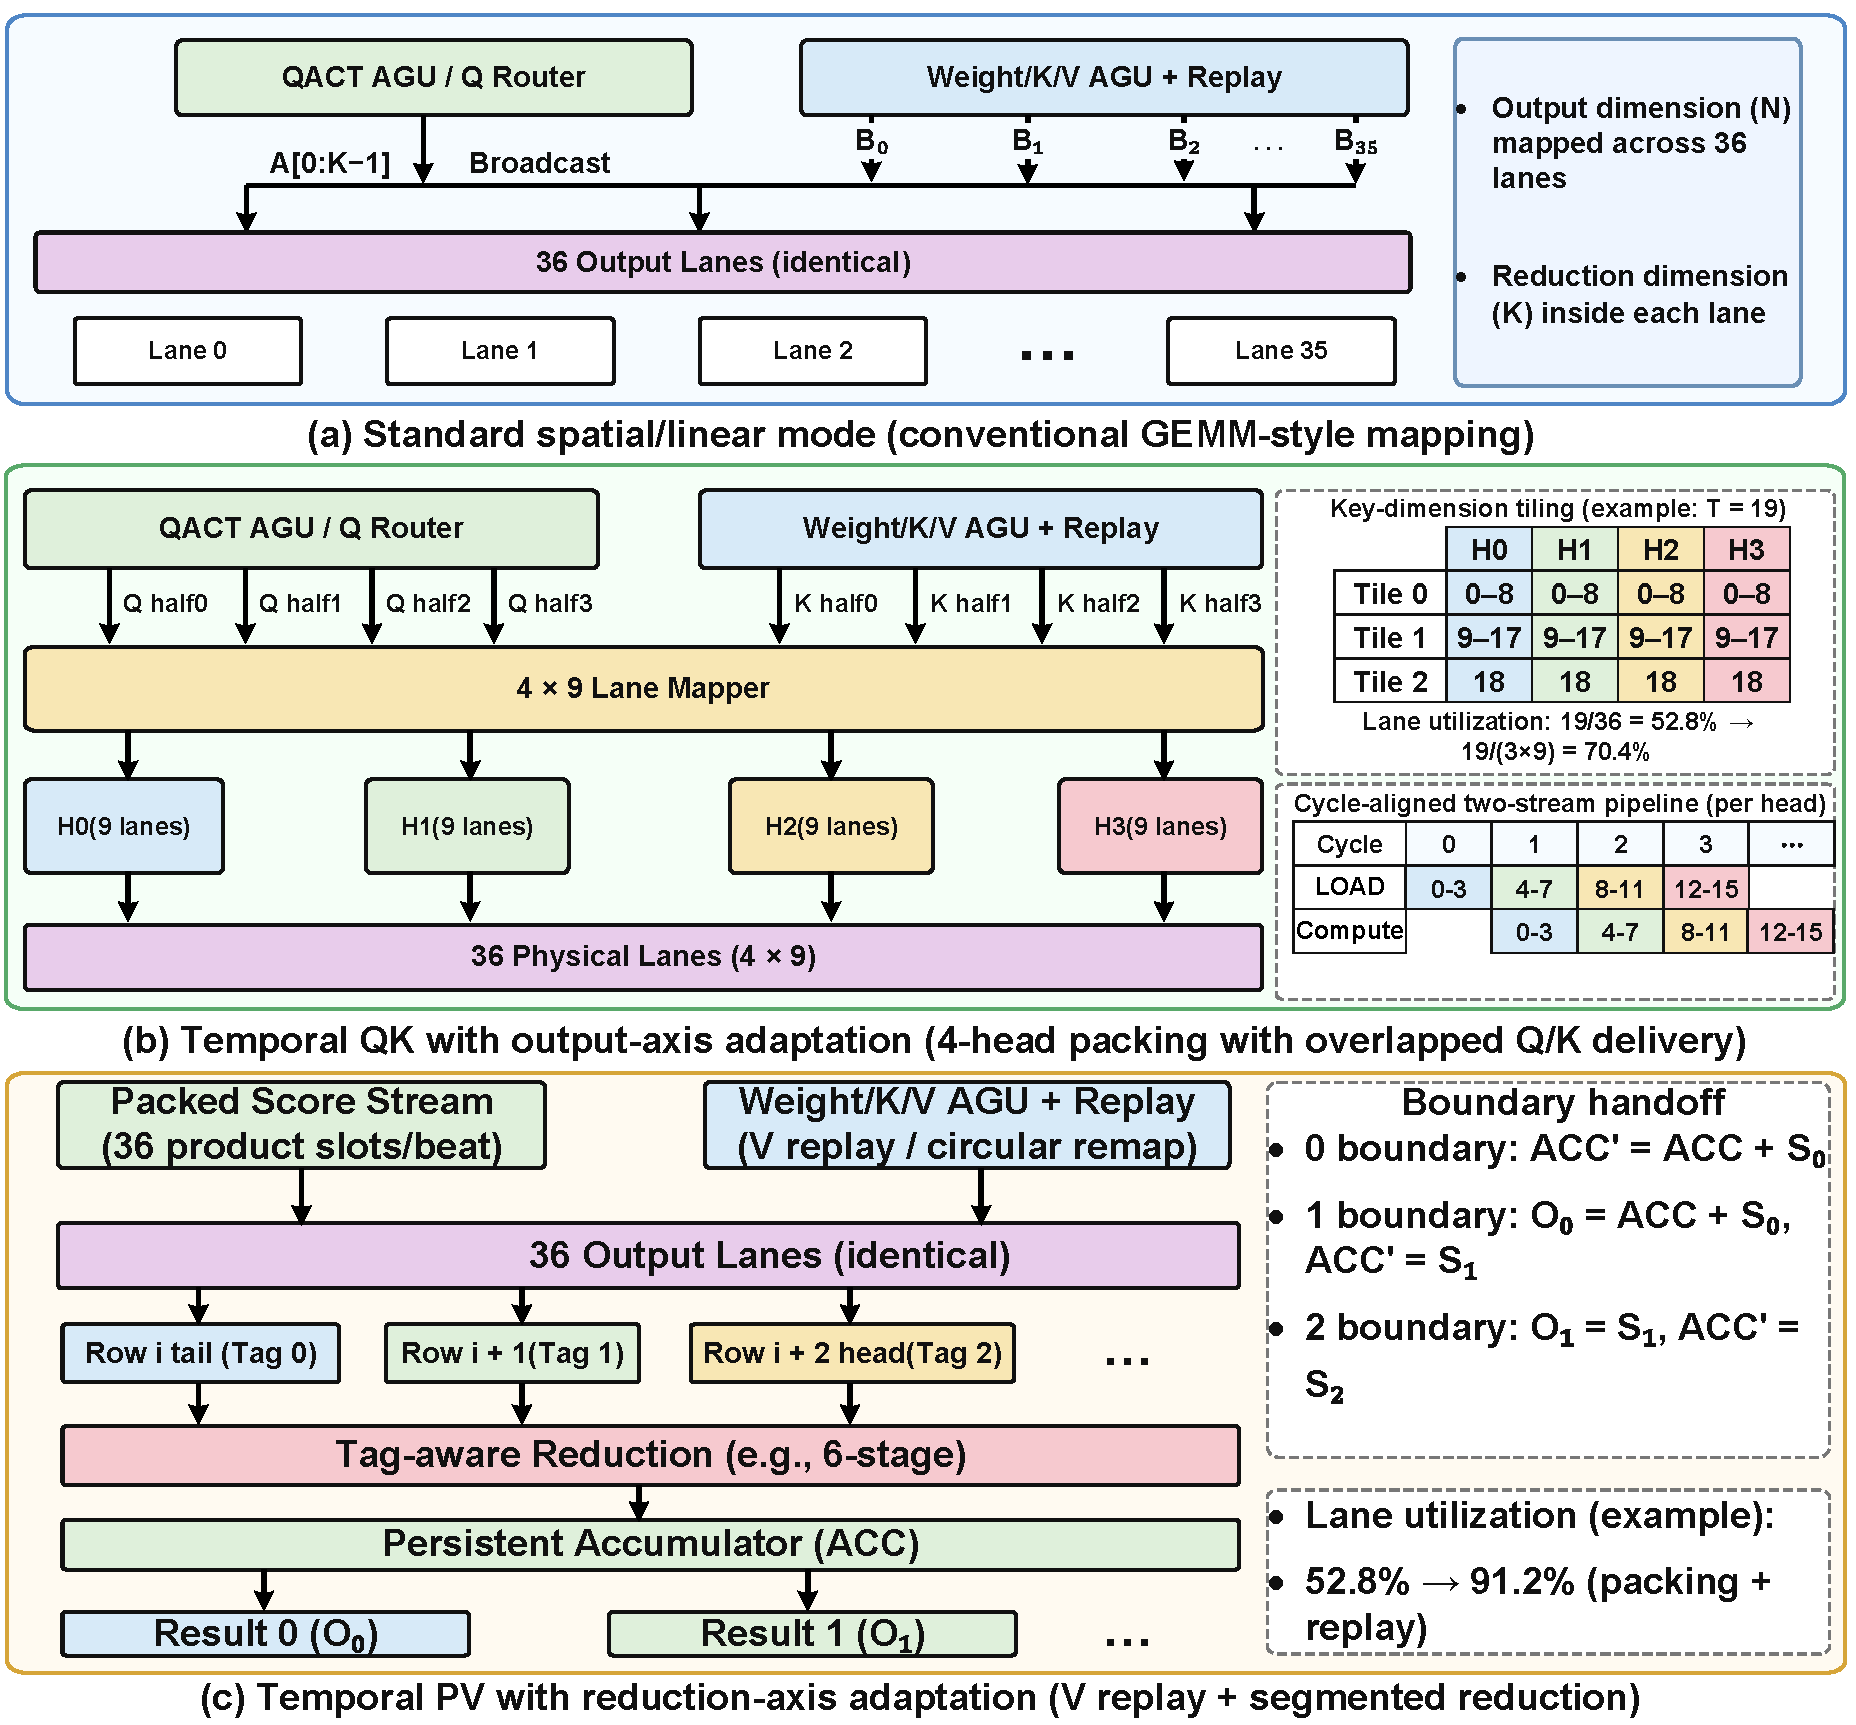
\includegraphics[width=\columnwidth]{fig/pea.pdf}
  \caption{Adaptive dataflows of the shared PEA:
  (a) conventional mapping;
  (b) temporal $QK^{\mathsf T}$ with four 9-lane head groups; and
  (c) temporal $PV$ with V replay and segmented reduction.}
  \label{fig:dare_modes}
  \vspace{-6mm}
\end{figure}

In $PV$, the temporal dimension becomes the reduction axis.
For $T=19$, conventional execution pads each row to the 36-product
reduction width, using only $19/36=52.8\%$ of the product slots.
As shown in Fig.~\ref{fig:dare_modes}(c), DARE instead packs adjacent
rows into a continuous product stream and replays the corresponding
$V$ entries to preserve score--value alignment.
Row tags steer a tag-aware reduction tree, while a persistent
accumulator carries partial sums across beat boundaries; dual-result
writeback handles beats that complete multiple rows.

For one output channel of a temporal-attention head, the 19 query rows require $19^2=361$ products, which occupy only
$\lceil361/36\rceil=11$ packed beats, increasing product-slot
utilization to $361/(11\times36)=91.2\%$.
Thus, the same PEA supports both output-axis adaptation in
$QK^{\mathsf T}$ and reduction-axis adaptation in $PV$ without a
dedicated temporal engine.
% ======================================================================
\section{Evaluation}
\label{sec:eval}

\subsection{Experimental Setup}
\textbf{Algorithm.}
We evaluate Open-Sora v1.2 STDiT3-XL/2~\cite{zheng2024opensora} on VBench~\cite{huang2024vbench}. All quality runs generate 64-frame, $512\times512$ videos with 30 rectified-flow steps using the full VBench prompt set with identical seeds and sampling settings. We compare FP16, ViDiT-Q~\cite{zhao2025viditq} (linear-only W8A8),
TeaCache~\cite{liu2025teacache} (FP16 caching), FP-Ind. C+Q (FP-domain caching with W8A8 execution), FP-Ind. + Q-Calib. (further recalibrating the predictor in the quantized domain), and QAC. The last three configurations use identical W8A8 linear+attention quantization and recomputation budgets, isolating the effects of quantized-domain calibration and indicator alignment.


% Algorithm quality is evaluated using 64-frame, $512\times512$ videos with 30 rectified-flow steps under identical prompts and sampling settings. The 64--512-frame workloads are additionally used in the hardware evaluation to characterize accelerator behavior across temporal dimensions.

\textbf{Hardware.}
Q-DARE is synthesized using Synopsys Design Compiler with
TSMC 7\,nm technology libraries at 1\,GHz.
The reported 1.05\,mm$^2$ area and 614.4\,mW power cover the complete accelerator implementation,
including logic and SRAM macros. A cycle-level simulator models accelerator latency, including
QAC execution on the existing VCU/controller, which contributes
at most 0.03\% of the total generation latency across the
evaluated video lengths. We reimplement ViDA~\cite{ding2025vida} according to its published architecture and dataflow in the same simulator, and evaluate both accelerators on the same Open-Sora workloads at 1\,GHz with 256\,GB/s off-chip bandwidth. For area comparison,
Q-DARE uses the direct 7-nm synthesis result, whereas ViDA
is normalized from 32 nm to 7 nm using the scaling methodology
reported in the original work~\cite{ding2025vida}. For comparison with A100~\cite{nvidiaA100}, following EXION~\cite{heo2025exion}, we scale Q-DARE to match the dense INT8 peak compute capability of the A100-80GB, while constraining its aggregate off-chip bandwidth to the same bandwidth budget. Q-DARE latency and power are projected from our cycle-level/7-nm models, whereas A100 latency and power are measured on the same workloads.

% For A100 \cite{nvidiaA100}, following EXION~\cite{heo2025exion}, we scale the number of Q-DARE cores to match the GPU's equivalent peak compute capability under the same workload and bandwidth model, and compare the resulting projected accelerator performance with measured A100 execution on the same workloads.


\textbf{Metrics.} Step and video throughput are measured in STDiT steps/s and videos/s, respectively. Energy and area efficiency are defined as step throughput per power (steps/J) and video throughput per area (videos/s/mm$^{2}$), respectively.

\begin{figure}[!t]
  \centering
  % TODO: Update this figure to add the Naive Cache+Quant row.
  % Recommended rows:
  % Original / ViDiT-Q / TeaCache / Naive Cache+Quant / QAC.
  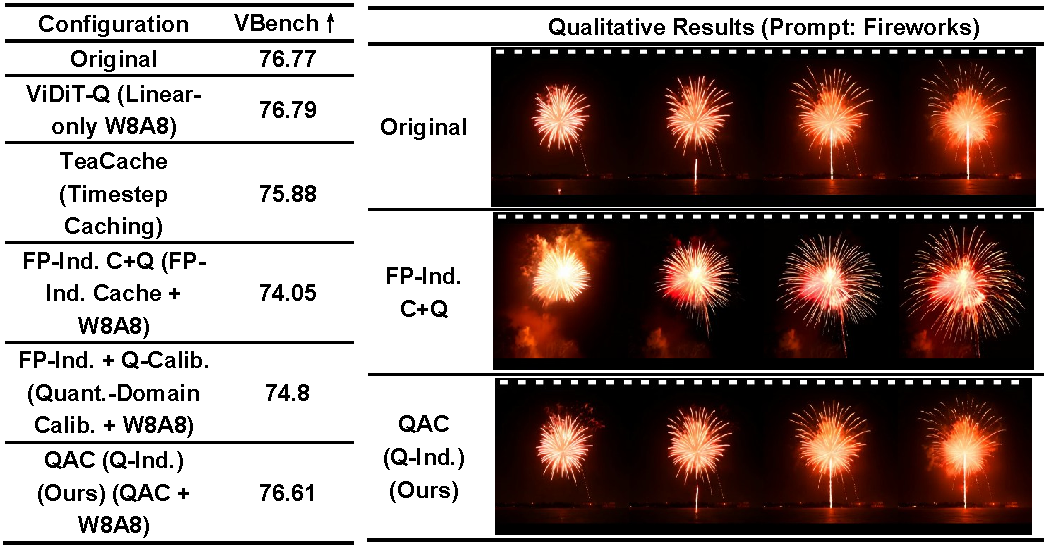
\includegraphics[width=\columnwidth]{fig/gen_img.pdf}
  % \caption{Open-Sora v1.2 quality comparison under identical prompts and sampling settings. Naive Cache+Quant and QAC use the same quantized execution and recomputation budget, differing only in the cache-indicator domain.}
  \caption{Open-Sora v1.2 quality comparison. Q-Calib. denotes predictor calibration in the quantized domain while retaining the FP indicator.}
  \label{fig:quality}
  \vspace{-4mm}
\end{figure}

\subsection{Algorithm Quality}
% Fig.~\ref{fig:quality} directly isolates the decision-domain mismatch. Under identical quantized execution and the same recomputation budget, Naive Cache+Quant reaches 74.05 VBench, whereas QAC recovers the score to 76.61. Q-DARE therefore remains only 0.16 below the FP16 baseline (76.77) while jointly applying timestep caching and quantized execution. ViDiT-Q and TeaCache separately show that quantization or caching alone does not capture this interaction.
As shown in Fig.~\ref{fig:quality}, quantized-domain calibration alone improves FP-Ind. C+Q from 74.05 to 74.80, while further aligning the indicator with quantized execution raises VBench to 76.61, only 0.16 below FP16. ViDiT-Q and TeaCache show the quality of quantization and caching when applied separately.

\subsection{Hardware Evaluation}
\textbf{Comparison with ViDA.}
Table~\ref{tab:vida_comparison} compares Q-DARE with our ViDA reimplementation under identical simulator, frequency, bandwidth, model, and workload settings. Q-DARE achieves \QDAREViDAThroughputGeo$\times$ geomean video throughput, with the gain increasing from 1.007$\times$ at 64 frames to 1.091$\times$ at 512 frames. Using video throughput per unit area, the direct 7-nm implementation result yields \QDAREViDAAreaGeo$\times$ geomean area efficiency.

\begin{table}[!t]
\centering
% \caption{Implementation characteristics and normalized comparison with ViDA.}
\caption{SYSTEM-LEVEL COMPARISON WITH VIDA.}
\label{tab:vida_comparison}
\scriptsize
\setlength{\tabcolsep}{3.0pt}
\renewcommand{\arraystretch}{1.02}
\resizebox{\columnwidth}{!}{%
\begin{tabular}{@{}ccc@{}}
\toprule
\textbf{Metric} & \textbf{Q-DARE} & \textbf{ViDA~\cite{ding2025vida}} \\
\midrule
\multicolumn{3}{c}{\textbf{Implementation Characteristics}} \\
\midrule
Technology & TSMC 7 nm & 32$\rightarrow$7 nm \\
Frequency & 1.0\,GHz & 1.0\,GHz \\
Precision & INT8/FP16 & FP16 \\
\multirow{2}{*}{Compute Units}
  & 1296 INT8 MACs & \multirow{2}{*}{640 FP16 MACs} \\
  & 36 FP16 MACs & \\
On-chip SRAM & 522.5\,KiB & N/R \\
Memory BW & 256\,GB/s & 256\,GB/s \\
Area (mm$^2$) & 1.05 & 2.03 \\
Power (mW) & 614.4 & N/R \\
\midrule
\multicolumn{3}{c}{\textbf{Normalized Results}} \\
\midrule
64F Video Throughput & 1.007$\times$ & 1.00$\times$ \\
256F Video Throughput & 1.071$\times$ & 1.00$\times$ \\
512F Video Throughput & 1.091$\times$ & 1.00$\times$ \\
Video Throughput Geomean & \textbf{\QDAREViDAThroughputGeo$\times$} & 1.00$\times$ \\
Area Eff. Geomean & \textbf{\QDAREViDAAreaGeo$\times$} & 1.00$\times$ \\
\bottomrule
\end{tabular}%
}
\vspace{0.5pt}
\parbox{\columnwidth}{\scriptsize
64F, 256F, and 512F denote video frames; all workloads use $512\times512$ resolution. Throughput and area efficiency are normalized to ViDA.}
\end{table}

\textbf{Comparison with A100.}
Fig.~\ref{fig:a100_comparison} compares STDiT step throughput and energy efficiency under the compute- and bandwidth-matched setting described above. Q-DARE provides 10.02--11.88$\times$ projected step-throughput speedup across the three video lengths, with a 10.96$\times$ geomean. Energy-efficiency gains range from 25.95$\times$ to 27.08$\times$, with a 26.59$\times$ geomean. The step-throughput metric isolates accelerator execution efficiency from the additional reduction in executed steps due to caching.

\begin{figure}[!t]
  \centering
  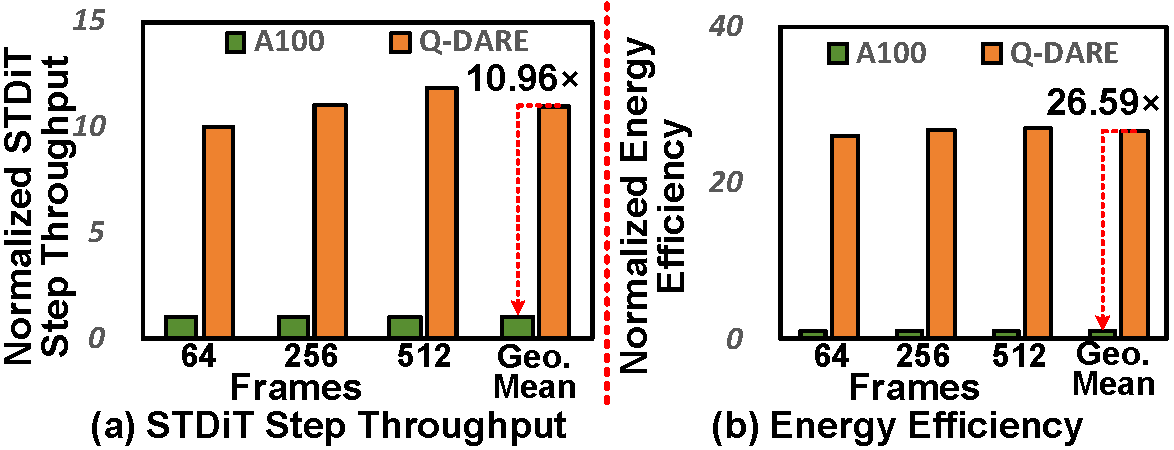
\includegraphics[width=\columnwidth]{fig/vs_A100.pdf}
  \caption{A100 comparison across video lengths: (a) normalized STDiT step throughput and
(b) normalized energy efficiency. A100 is normalized to 1.}
  \label{fig:a100_comparison}
  \vspace{-4mm}
\end{figure}

\begin{table}[!t]
\centering
\caption{Ablation of DARE on the shared PEA.}
\label{tab:dare_ablation}
\scriptsize
\setlength{\tabcolsep}{2.4pt}
\renewcommand{\arraystretch}{1.03}

\resizebox{\columnwidth}{!}{%
\begin{tabular}{@{}lcccccc@{}}
\toprule
\textbf{Configuration} &
\textbf{64F} &
\textbf{256F} &
\textbf{512F} &
\textbf{Geo.} &
\textbf{Area} &
\textbf{Area Eff.} \\
\midrule

Static mapping
& 1.00$\times$
& 1.00$\times$
& 1.00$\times$
& 1.00$\times$
& 0.985
& 1.00$\times$ \\

+ $QK^{\mathsf T}$ output-axis adapt.
& 1.14$\times$
& 1.14$\times$
& 1.08$\times$
& 1.12$\times$
& 0.993
& 1.11$\times$ \\

+ $PV$ reduction adapt.
& 1.50$\times$
& 1.37$\times$
& 1.18$\times$
& 1.34$\times$
& 1.051
& 1.26$\times$ \\
\bottomrule
\end{tabular}%
}

\vspace{1pt}
\raggedright
\scriptsize
Speedup is normalized to static mapping; Geo. is the geometric mean;
Area is in mm$^2$; Area Eff. is normalized throughput per unit area.
\vspace{-4mm}
\end{table}

\textbf{DARE ablation.}
Table~\ref{tab:dare_ablation} evaluates the performance--area trade-off of the adaptive dataflows.
Output-axis adaptation achieves 1.12$\times$ geomean speedup with only 0.8\% estimated total-area overhead.
Full DARE increases the speedup to 1.34$\times$ with 6.7\% area overhead, yielding 1.26$\times$ area efficiency over static mapping.
The gain is largest for the 64-frame workload ($T=19$), where short temporal dimensions cause the strongest underutilization.

% ======================================================================
\section{Conclusion}
\label{sec:conclusion}

Q-DARE co-designs cache decisions and attention execution for low-precision video diffusion. QAC aligns reuse decisions with the quantized trajectory, while DARE adapts a shared PEA along the output and reduction axes of factorized attention. On Open-Sora v1.2, Q-DARE achieves 76.61 VBench
(76.77 for FP16), 10.96$\times$ STDiT throughput and
26.59$\times$ energy efficiency over A100, and
1.06$\times$ video throughput and 2.04$\times$ area
efficiency over ViDA.

\clearpage
\bibliographystyle{IEEEtran}
\bibliography{references}

\end{document}
